\let\negmedspace\undefined
\let\negthickspace\undefined
\documentclass[journal]{IEEEtran}
\usepackage[a5paper, margin=10mm, onecolumn]{geometry}
%\usepackage{lmodern} % Ensure lmodern is loaded for pdflatex
\usepackage{tfrupee} % Include tfrupee package

\setlength{\headheight}{1cm} % Set the height of the header box
\setlength{\headsep}{0mm}     % Set the distance between the header box and the top of the text

\usepackage{gvv-book}
\usepackage{gvv}
\usepackage{cite}
\usepackage{amsmath,amssymb,amsfonts,amsthm}
\usepackage{algorithmic}
\usepackage{graphicx}
\usepackage{textcomp}
\usepackage{xcolor}
\usepackage{txfonts}
\usepackage{listings}
\usepackage{enumitem}
\usepackage{mathtools}
\usepackage{gensymb}
\usepackage{comment}
\usepackage[breaklinks=true]{hyperref}
\usepackage{tkz-euclide} 
\usepackage{listings}
% \usepackage{gvv}                               

\def\inputGnumericTable{}                      
\usepackage[latin1]{inputenc}                    
\usepackage{color}                              
\usepackage{array}                             
\usepackage{longtable}                          
\usepackage{calc}                               
\usepackage{multirow}                           
\usepackage{hhline}                            
\usepackage{ifthen}                          
\usepackage{lscape}
\begin{document}

\bibliographystyle{IEEEtran}
\vspace{3cm}

\title{3.3.8}
\author{AI25BTECH11024 - Pratyush Panda
}
\maketitle
% \newpage
% \bigskip
{\let\newpage\relax\maketitle}

\renewcommand{\thefigure}{\theenumi}
\renewcommand{\thetable}{\theenumi}
\setlength{\intextsep}{10pt} % Space between text and floats


\numberwithin{equation}{enumi}
\numberwithin{figure}{enumi}
\renewcommand{\thetable}{\theenumi}

\textbf{Question: } \\
Construct a triangle $\Delta ABC$ with side $BC = 7 cm$, $\angle B=45^\circ$, $\angle A=105^\circ$.
\vspace{0.7cm}

\textbf{Solution: } \\
Let the position vector of $\Vec{B}$ be $\myvec{0 \\ 0}$ and the position vector of $\Vec{C}$ be $\myvec{7 \\ 0}$ as $BC=7cm$ is given.\\
Let a, b and c be the length of sides opposite to the vertex A, B and C respectively.

Now, we know that sum of all interior angles of a triangle is $180^\circ$, thus;
\begin{align}
\angle A + \angle B + \angle C = 180^\circ
\end{align}
\begin{align}
or \, 105^\circ + 45^\circ + \angle C = 180^\circ
\end{align}
\begin{align}
Thus, \, \angle C = 30^\circ
\end{align}

We can form two equations to get the other two sides such as;
\begin{align}
b\cos C + c\cos B = 8
\end{align}
\begin{align}
b\sin C - c\sin B = 0
\end{align}

On writing this system of equation as a matrix equation, we get;
\begin{align}
\myvec{\cos C & \cos B \\
       \sin C & -\sin B}
\Vec{X} = 
\myvec{7 \\ 0} \, \textit{where } \Vec{X}=\myvec{b \\ c}
\end{align}

After putting the values of all the trigonometric values, we get;
\begin{align}
\myvec{\frac{\sqrt{3}}{2} & \frac{1}{\sqrt{2}} \\
       \frac{1}{2} & -\frac{1}{\sqrt{2}}}
\Vec{X} = 
\myvec{7 \\ 0}
\end{align}

Now we can do row operations to get the Echelon form of this matrix.
\begin{align}
\myvec{\sqrt{3}/2 & 1/\sqrt{2} \\
    0 & (-\frac{1}{\sqrt{2}} - \frac{1}{\sqrt{6}}}
\Vec{X} = 
\myvec{7 \\ \frac{7}{\sqrt{3}}}
\end{align}

On solving this equation we get;
\begin{align}
\Vec{X} = \myvec{7\brak{\frac{1-\sqrt{3}}{\sqrt{3}}} \\ \frac{7\sqrt{2}}{\sqrt{3}-1}}
\end{align}

From here we get, $c=\frac{7\sqrt{2}}{\sqrt{3}-1}$ \\

Now, the coordinates of $\Vec{A}$ can be written as;
\begin{align}
\Vec{A}=\myvec{c\cos B \\ c\sin B}
\end{align}
\begin{align}
or, \, \Vec{A}=\myvec{\frac{c}{\sqrt{2}} \\ \frac{c}{\sqrt{2}}}=\myvec{\frac{7}{\sqrt{3}-1} \\ \frac{7}{\sqrt{3}-1}}
\end{align}
Now, we can plot the triangle using the three points.

\begin{figure}[H]
\centering
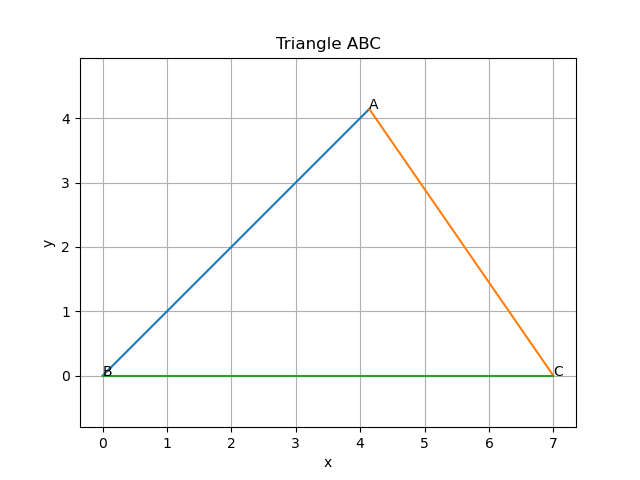
\includegraphics[width=0.8\columnwidth]{figs/img.png}
\caption*{}
\end{figure}

\end{document}